\subsection{Dataset and variables}

The study uses an internal corrosion database from a producing oil field: 903 raw records of measured corrosion rates, along with the operating conditions, produced-water chemistry, production rates, and service time for each monitoring point. Data preparation removed six records with physically invalid negative rates and the columns identified by the leakage audit of Section~\ref{sec:vmod}, leaving 897 records and 31 candidate variables. Missing entries received the training-fold median inside each cross-validation fold.

Table~\ref{tab:features} describes every variable considered with its physical meaning and unit. The set covers the CO$_2$-corrosion driving forces ($p_{\mathrm{CO_2}}$, $y_{\mathrm{CO_2}}$, $T$, $P$, pH), the water chemistry that controls scaling and conductivity ($[\mathrm{HCO_3^-}]$, $[\mathrm{Ca^{2+}}]$, $[\mathrm{Cl^-}]$, $\sigma$, TDS, Alk), the hydrodynamic and production variables that control wall shear and phase wetting ($u$, $Q_w$, $Q_o$, $Q_g$, FP), the solids content associated with under-deposit attack (TSS), and the service time $t_s$, which is fixed at installation and therefore known before any inspection.

\begin{table}[htb!]
\centering
\footnotesize
%\setlength{\tabcolsep}{2pt}
\caption{Variables of the dataset: physical meaning, units and descriptive statistics (897 records; the measured rate $v$ is reported after saturation at 20 [mpy]).}
\label{tab:features}
\begin{tabularx}{0.45\textwidth}{@{}lX@{}}
\toprule
Symbol & Meaning [unit]\\%& Min & Median & Mean & Max & Missing \\
\midrule
\midrule
$v$ & measured corrosion rate [mpy] \\%& 0 & 5.26 & 8.38 & 20 & 0 \\
$t_s$ & service time of the monitoring point [yr] \\%& -0.0219 & 9.83 & 11.8 & 38.1 & 0 \\
$p_{\mathrm{CO_2}}$ & CO$_2$ partial pressure [psig] \\%& 0 & 12 & 17.2 & 103 & 13 \\
$y_{\mathrm{CO_2}}$ & CO$_2$ gas mole fraction [--] \\%& 0 & 16 & 22.7 & 52.5 & 13 \\
$y_{\mathrm{CH_4}}$ & methane gas mole fraction [--] \\%& 0 & 46.7 & 45.6 & 87.7 & 15 \\
$y_{\mathrm{N_2}}$ & nitrogen gas mole fraction [--] \\%& -6.32 & 13.2 & 17 & 78.4 & 15 \\
$u$ & production fluid velocity [ft/s] \\%& 0 & 4.57 & 5.29 & 32.5 & 31 \\
$P$ & operating pressure [psig] \\%& 0 & 66 & 72.2 & 231 & 0 \\
$T$ & operating temperature [$^{\circ}$F] \\%& 0 & 248 & 233 & 250 & 0 \\
pH & produced-water pH [--] \\%& 0.23 & 6.85 & 6.93 & 7.88 & 14 \\
$\sigma$ & water electrical conductivity [$\mu$S/cm] \\%& -325 & 529 & 603 & 5.78e+03 & 13 \\
$[\mathrm{Cl^-}]$ & chloride concentration [ppm] \\%& -19 & 9.96 & 30.7 & 752 & 14 \\
$[\mathrm{Na^+}]$ & sodium concentration [ppm] \\%& -28.3 & 68.7 & 79.5 & 302 & 15 \\
$[\mathrm{Ca^{2+}}]$ & calcium concentration [ppm] \\%& 0.072 & 11.6 & 16.2 & 117 & 14 \\
$[\mathrm{Mg^{2+}}]$ & magnesium concentration [ppm] \\%& 0 & 4.9 & 4.54 & 12.3 & 14 \\
$[\mathrm{Ba^{2+}}]$ & barium concentration [ppm] \\%& 0 & 0.23 & 0.415 & 5.27 & 14 \\
$[\mathrm{Sr^{2+}}]$ & strontium concentration [ppm] \\%& 0 & 0.227 & 4.88 & 752 & 14 \\
$[\mathrm{Fe}]$ & total dissolved iron [ppm] \\%& -8.1 & 0.984 & 2.87 & 17.4 & 14 \\
$[\mathrm{SO_4^{2-}}]$ & sulfate concentration [ppm] \\%& -2.73 & 7.41 & 25.9 & 496 & 14 \\
$[\mathrm{HCO_3^-}]$ & bicarbonate concentration [meq/L] \\%& 1.96 & 4 & 110 & 361 & 14 \\
Alk & total alkalinity [ppm CaCO$_3$] \\%& -4 & 219 & 207 & 580 & 14 \\
TH & total hardness [ppm CaCO$_3$] \\%& 0 & 27.8 & 43.3 & 291 & 14 \\
TSS & total suspended solids [ppm] \\%& -123 & 64 & 76.2 & 437 & 14 \\
TDS & total dissolved solids [ppm] \\%& 248 & 347 & 385 & 2.03e+03 & 14 \\
$Q_w$ & water production rate [BWPD] \\%& 0 & 6.33e+03 & 8.48e+03 & 7.79e+04 & 0 \\
$Q_o$ & oil production rate [BOPD] \\%& 0 & 68.2 & 89.2 & 981 & 0 \\
$Q_g$ & gas production rate [MMSCFD] \\%& 0 & 3.29e-09 & 786 & 2.95e+04 & 0 \\
FP & flow-pattern class [--] \\%& 0 & 2 & 1.76 & 3 & 13 \\
$D$ & nominal pipe diameter [in] \\%& 3 & 4 & 4.43 & 18 & 0 \\
$D_i$ & internal pipe diameter [in] \\%& 2.07 & 3.07 & 3.16 & 17.2 & 43 \\
$D_e$ & external pipe diameter [in] \\%& 2 & 4.5 & 4.68 & 18 & 0 \\
$e$ & wall thickness [mm] \\%& 2.87 & 5.49 & 5.75 & 9.53 & 0 \\
\bottomrule
\end{tabularx}
\end{table}


\subsection{Leakage audit and excluded variables}
\label{sec:vmod}

The raw database carries a column of calculated corrosion rate, obtained from the inspection record of each monitoring point as the average thickness-loss rate over the service life,
\begin{equation}
  v_{\mathrm{calc}} = \frac{(e - e_{\min})}{t_s}
                      \cdot \frac{1000}{25.4},
  \label{eq:vmod}
\end{equation}
where $e$ [mm] is the reference wall thickness, $e_{\min}$ [mm] the minimum wall thickness measured at the point, $t_s$ [yr] the service time, and the factor $1000/25.4$ converts [mm/yr] to [mpy].  

The study consequently excludes from the candidate variables: the minimum thickness $e_{\min}$, which requires the same inspection that defines the target; the wear and remaining-life columns derived from them; and the failure flag, which labels the record itself as a failure event --- an outcome unknown at prediction time. The service time $t_s$ remains fixed at installation, known before any measurement campaign, and enters as a regular covariate of exposure.
\subsection{Normative segmentation and target treatment}

The normative limits $\{2, 8\}$ [mpy] partition the target into three classes: low $(0,2]$, medium $(2,8]$, and high $(>8)$. Table~\ref{tab:classes} reports the class distribution and Figure~\ref{fig:hist} the target histogram. For the regression task, the target saturates at 20 [mpy], which is 2.5 times the highest normative limit; above this level, all integrity decisions are identical (immediate intervention), so prediction error beyond this level carries no operational meaning. The saturation affects 176 records (19.6\%). A variance analysis motivates this treatment: on the raw target, a hypothetical perfect three-class predictor mapped to class medians cannot exceed a coefficient of determination of 0.46, because a small number of extreme rates (up to 322 [mpy]) dominates the total variance. Classification remains unaffected, since both normative limits lie far below the saturation level. Every model in the study, including the benchmarks, trains and evaluates on the saturated target.

\begin{table}[htb!]
\centering
\footnotesize
\setlength{\tabcolsep}{4pt}
\caption{Distribution of the records across the normative severity classes [mpy].}
\label{tab:classes}
\begin{tabular}{@{}cccc@{}}
\toprule
$n$ & low $(0,2]$ & mid $(2,8]$ & high $(>8)$ \\
\midrule
\midrule
897 & 223 & 309 & 365 \\
\bottomrule
\end{tabular}
\end{table}


\begin{figure}[htb!]
  \centering
  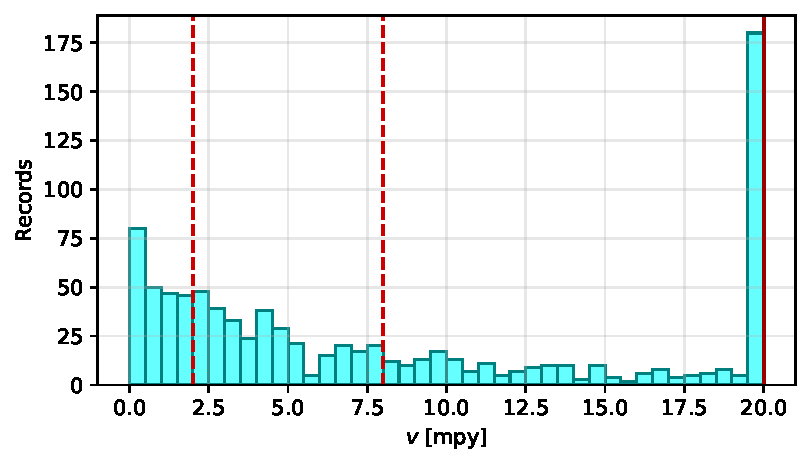
\includegraphics[width=0.9\linewidth]{figures/hist_target.pdf}
  \caption{Distribution of the measured corrosion rate after
    saturation. Dashed lines mark the normative limits at 2 [mpy] and
    8 [mpy]; the solid line marks the saturation level at 20 [mpy].}
  \label{fig:hist}
\end{figure}


